\section{PPReCOGG: A Model for the Per-Pixel Classification of Early Breast Lesions via Gabor Features}

\subsection{PPReCOGG Classifies Sub-Regions of Perceptibly Distinct Textures in Synthetic Benchmarks}

To assess the baseline ability of the PPReCOGG model to distinguish natural patterns from one-another, the PPReCOGG model was trained and benchmarked against the Brodatz textures (namely the ``Raffia'' and ``Brick'' textures) compiled in the USC-SIPI image dataset, which is a common image dataset used in the evaluation of image processing and texture recognition community \citep{weber1997}. The brick and raffia textures were selected as they are visually distinct, and test images comprised of sub-regions of the two are perceptibly distinct upon visual inspection (\emph{Table 3.1a}).\par

Three-dimensional  multidimensional scaling (MDS) embeddings of the forty-eight-dimensional Gabor energy features calculated from the Brick and Raffia Brodatz textures reveal that while they intersects, the feature embeddings describe two distinct planes, each belonging to one of the two classes (\emph{Figure \ref{embeddings}a}).

The PPReCOGG model achieved high average accuracy rates of 90\% in benchmarks consisting of the Raffia and Brick Wall Brodatz textures (\emph{Table 3.1}).\par


\begin{figure}[p]
	\begin{center}
	\caption{MDS Embedding of Gabor Energy Features from Brodatz and Early Human Breast Lesion Datasets \label{embeddings}}
	\end{center}
	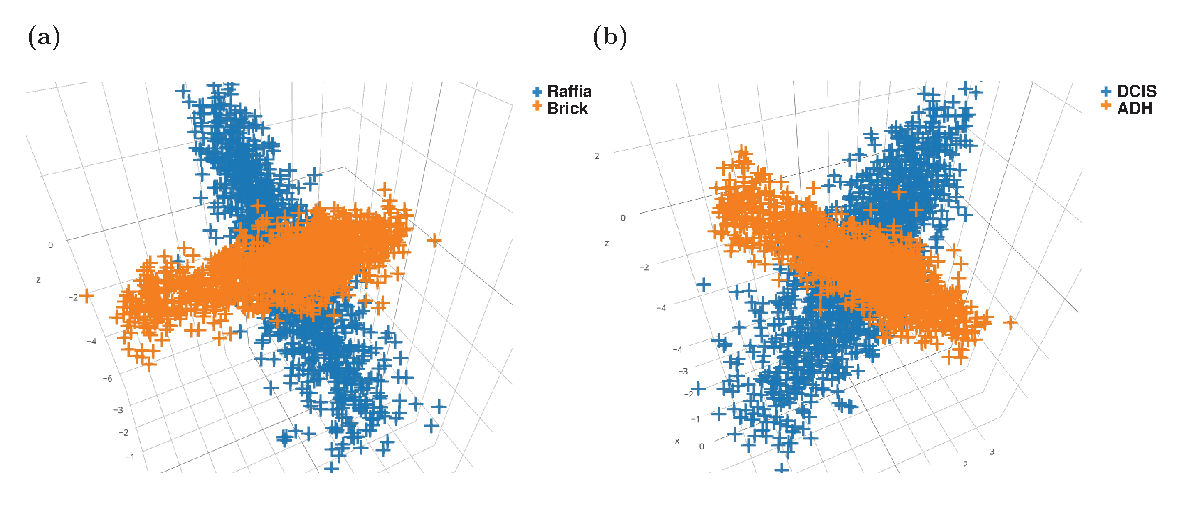
\includegraphics[width=170mm]{figures/embeddings/figure.pdf}
	 \begin{singlespace}
	 	\textit{Legend} --- Three-dimensional multidimensional scaling (MDS) embedding of Gabor energy features from known classes of the \textbf{(a)} Brodatz dataset and \textbf{(b)} the early human breast lesion dataset.
	 \end{singlespace}
	
\end{figure}


\clearpage

\begin{minipage}{\linewidth}
	\begin{center}
	
		\captionof{table}{Accuracy of the PPReCOGG Model Trained on Brodatz Textures 	\label{tab:brodatzclassify} }
		\begin{tabular}{>{\bfseries\centering}m{0.2in} >{\centering\bfseries}m{1in} >{\centering}m{1in} >{\centering}m{1in} >{\centering\arraybackslash}m{1in}}
			\hline
			&
			&
			\textbf{Test Image One}
			&
			\textbf{Test Image Two}
			&
			\textbf{Test Image Three}
			\\ 
			\hline
			(a)
			&
			Original
			&
			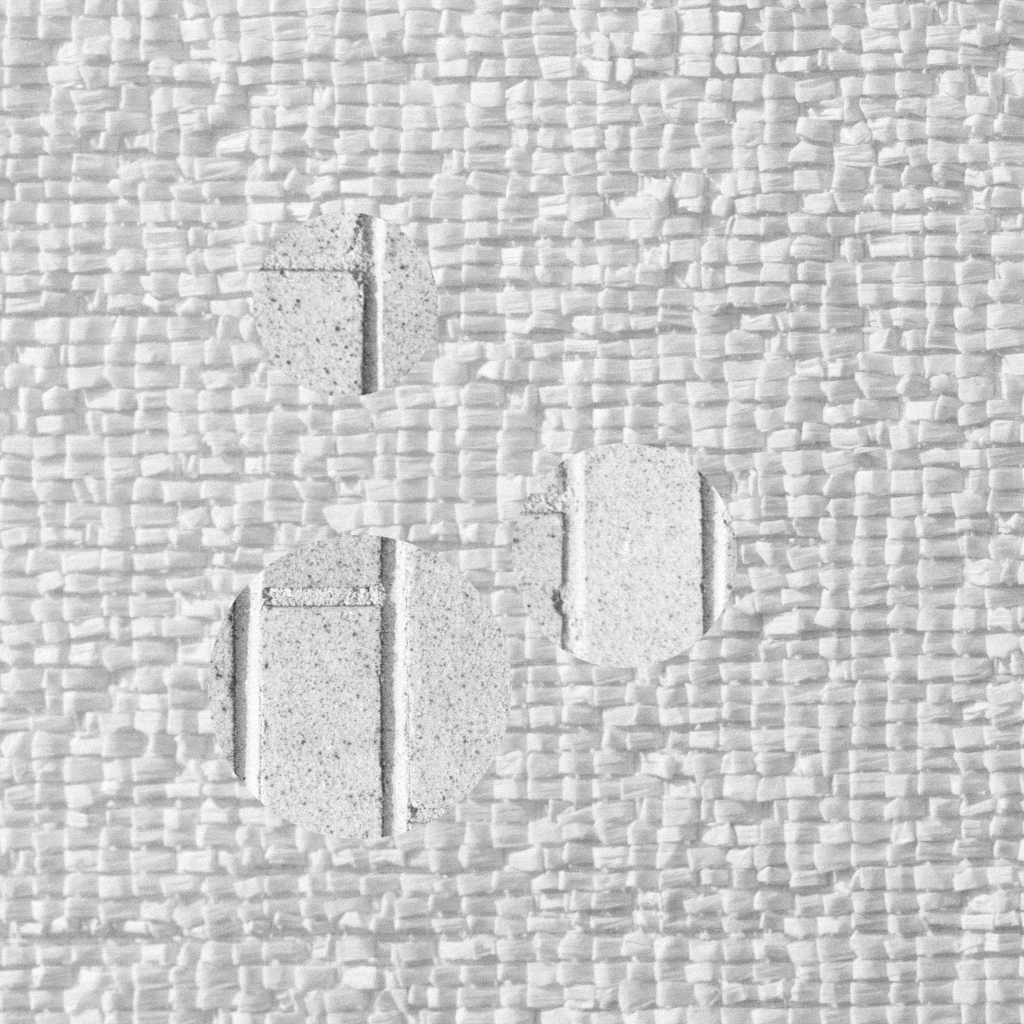
\includegraphics[width=75px, frame]{figures/accuracy_maps/original_brick_gravel_01.png}
			&
			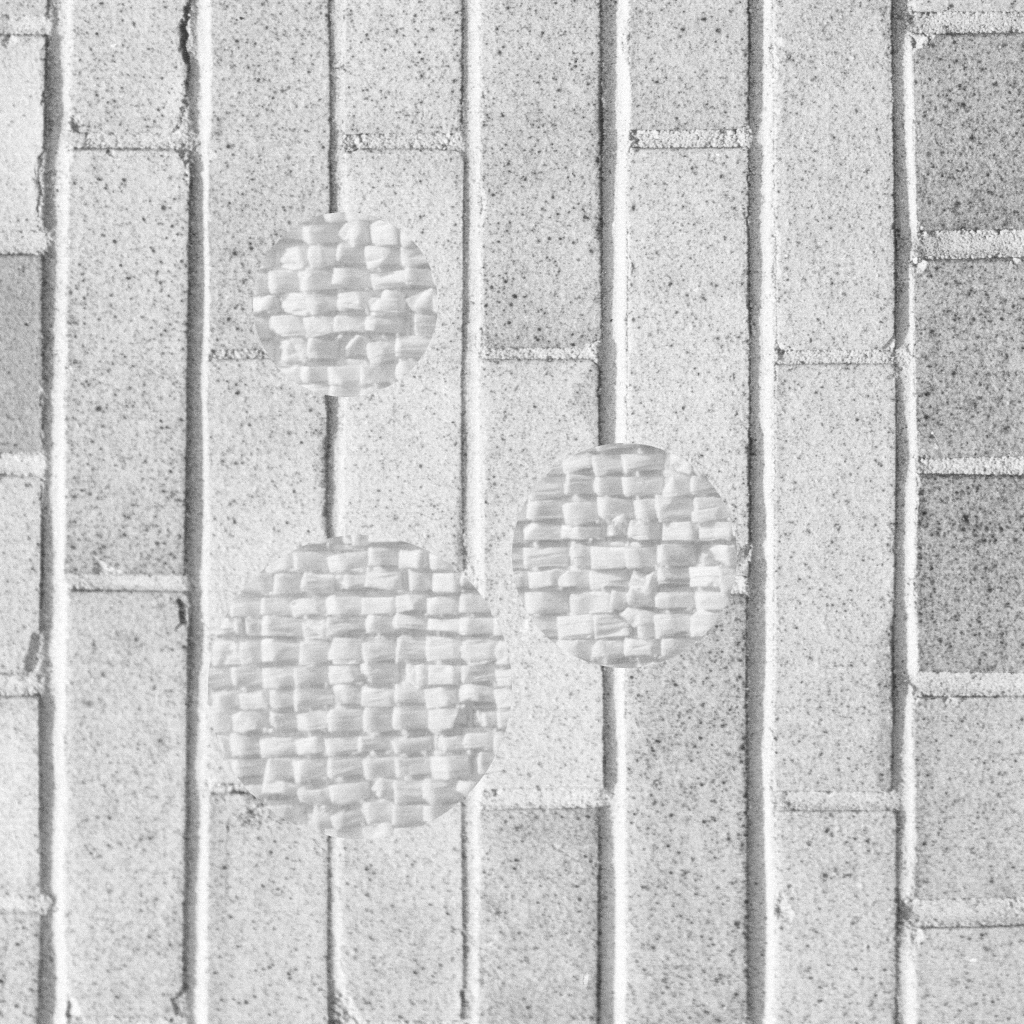
\includegraphics[width=75px, frame]{figures/accuracy_maps/original_brick_gravel_02.png}
			& 
			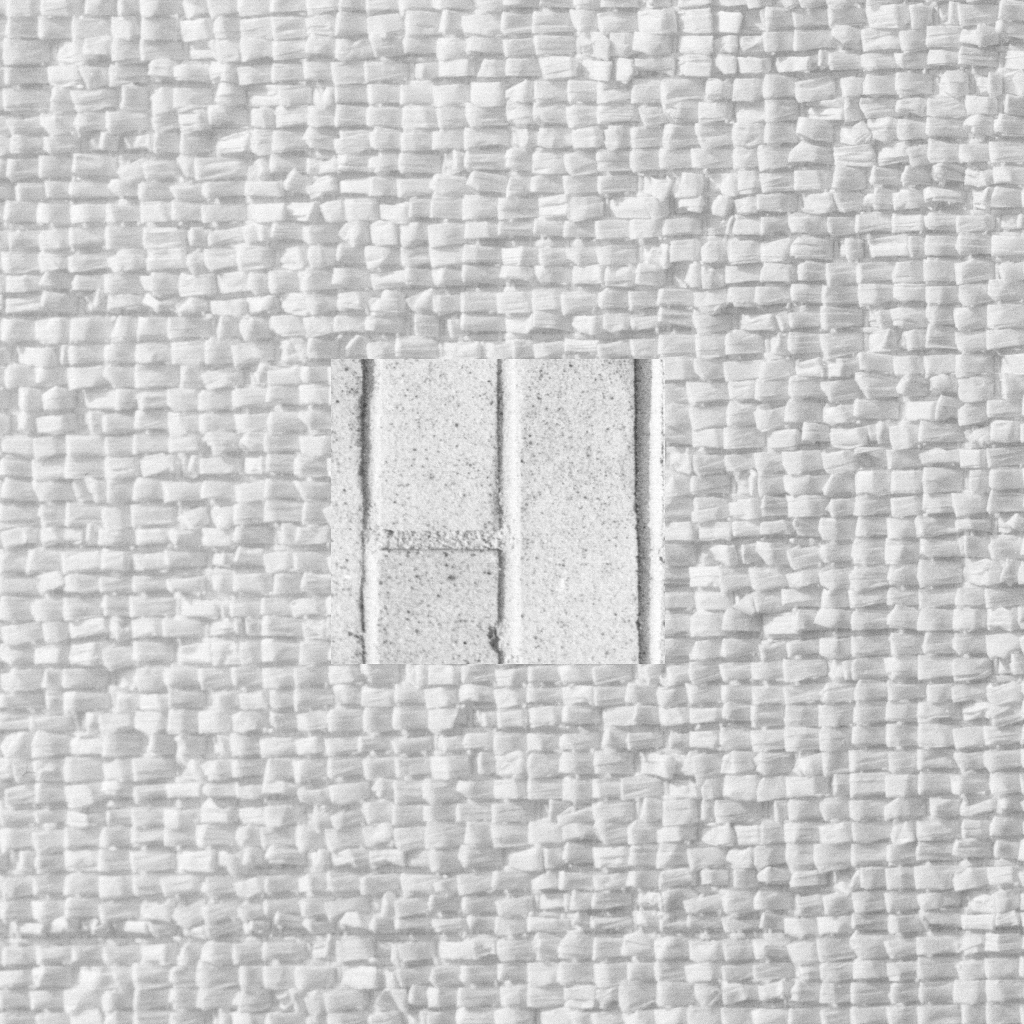
\includegraphics[width=75px, frame]{figures/accuracy_maps/original_brick_gravel_03.png}
			\\ 
			\hline
			(b)
			&
			Ground Truth
			&
			
\includegraphics[width=75px, frame]{figures/accuracy_maps/ground_truth_brick_gravel_01.png}
			&
			
\includegraphics[width=75px, frame]{figures/accuracy_maps/ground_truth_brick_gravel_02.png}
			& 
			
\includegraphics[width=75px, frame]{figures/accuracy_maps/ground_truth_brick_gravel_03.png}
			\\
			\hline
			(c)
			&
			Classified Image
			&
			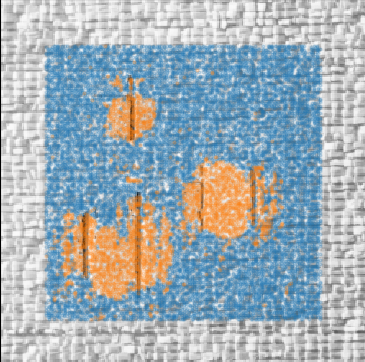
\includegraphics[width=75px, frame]{figures/accuracy_maps/brick_gravel_01_overlay_tight.png}
			&
			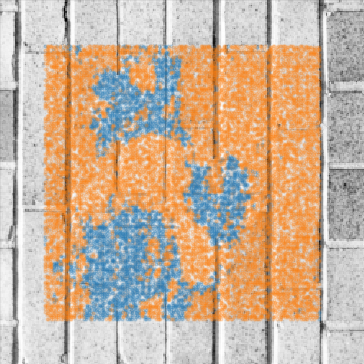
\includegraphics[width=75px, frame]{figures/accuracy_maps/brick_gravel_02_overlay_tight.png}
			&
			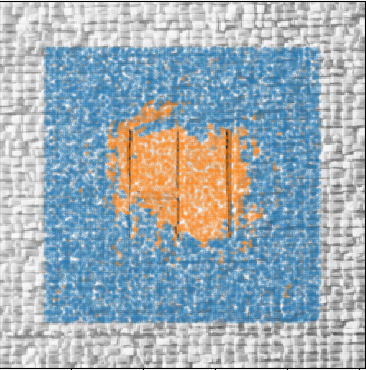
\includegraphics[width=75px, frame]{figures/accuracy_maps/brick_gravel_03_overlay_tight.png}
			\\
			\hline
			(d)
			&
			Raffia Accuracy Map
			&
			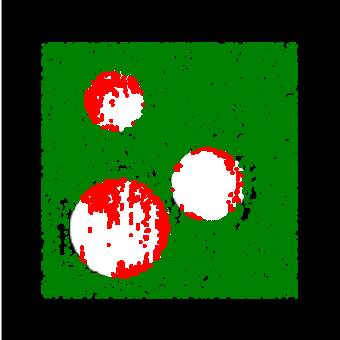
\includegraphics[width=75px, frame]{figures/accuracy_maps/brick_gravel_01_gravel_92_5.pdf}
			&
			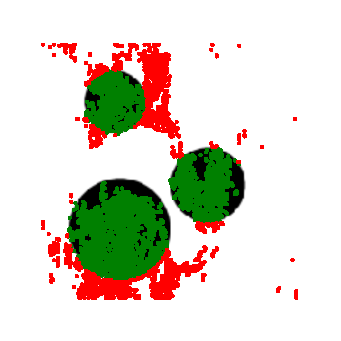
\includegraphics[width=75px, frame]{figures/accuracy_maps/brick_gravel_02_gravel.pdf}
			&
			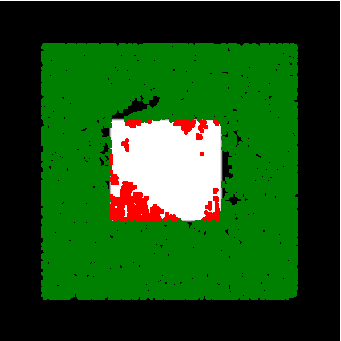
\includegraphics[width=75px, frame]{figures/accuracy_maps/brick_gravel_03_gravel.pdf}
			\\
			\hline
			(e)
			&
			Brick Accuracy Map
			&
			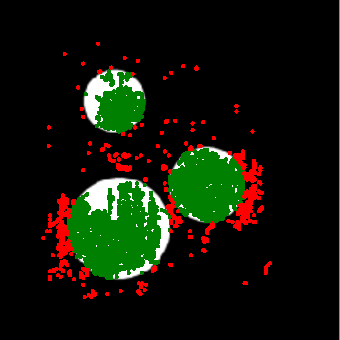
\includegraphics[width=75px, frame]{figures/accuracy_maps/brick_gravel_01_brick_84_6.pdf}
			&
			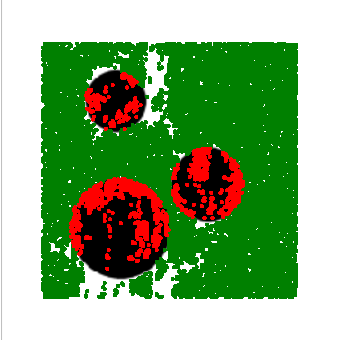
\includegraphics[width=75px, frame]{figures/accuracy_maps/brick_gravel_02_brick.pdf}
			&
			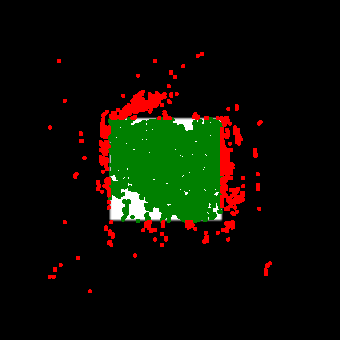
\includegraphics[width=75px, frame]{figures/accuracy_maps/brick_gravel_03_brick.pdf}
			\\ 
			\hline
			(f)
			&
			Accuracy
			&
			90.94\%
			&
			85.29\%
			&
			94.00\% 
			\\
			\hline
		\end{tabular}\par
	\end{center}
	\bigskip
	\begin{singlespace}
		\textit{Legend} --- \textbf{(a)} Test images comprised of composites of the Brodatz textures entitled ``Raffia'' (pg. D84) and ``Brick Wall'' (pg. D94). \textbf{(b)} The ideal classification (or ``ground truth'') of the original test image, where black pixels code for the raffia texture and white codes for the brick texture. \textbf{(c)} A random sampling of pixels classified by the PPReCOGG model. Pixels classified as Raffia are coded by blue points, and and pixels classified as Brick are coded by orange pixels. \textbf{(d)} and \textbf{(e)} Classified pixels are here compared to and overlayed on their ground truth. Pixels which are correctly classified are coded in green, while false-positives are coded in red. \textbf{(f)} Accuracy of the model, as calculated by the quotient of the number of correctly classified pixels and the total number of classified pixels. \label{brodatz_benchmark}
	\end{singlespace}
\end{minipage}



\subsection{PPReCOGG Classifies Sub-Regions of Different Neoplastic Phenotypes in Synthetic Benchmarks with High Accuracy}
\label{sec:synth_human}

Similar benchmarks were performed on test patterns composed of images of early lesions (ADH and DCIS) from human patient samples which had been immunofluorescently labelled for E-cadherin. These synthetic benchmarks are meant to simulate and quantitatively measure the efficiency of the PPReCOGG model in the task of classifying whole fields into sub-regions which exhibit cell patterning characteristic to certain early lesions.\par

MDS embeddings of the 48-dimensional Gabor energy features for the human samples reveal results very similar to the embeddings of the features of the Brodatz textures; two distinct but intersecting planes (\textit{Figure \ref{embeddings}b}).\par

The PPReCOGG model achieved high accuracy rates on the human lesion benchmarks, achieving an accuracies ranging from 93.17\% to 96.00\% across all test images (\textit{Table \ref{human_lesion}}).\par



\subsection{PPReCOGG Effectively Classifies Sub-Regions of Different Neoplastic Phenotypes in Human Biopsy Samples}

PPReCOGG model trained on E-cadhering patterning found in early breast lesion phenotypes (same features as those used in \S\ref{sec:synth_human}, see \textit{Figure \ref{fig:pprecogg_human_lesion}a}). This model was subsequently used to classify the pixels in images of early human breast lesions in with \mbox{E-cadherin} had been immunofluorescently labelled (\textit{Figure \ref{fig:pprecogg_human_lesion}b}). PPReCOGG effectively classifies sub-regions within the image that exhibit different cell-patterning characteristically found in early lesions.\par

\begin{minipage}{\linewidth}
	\begin{center}
		\label{tab:human_lesion} 
		\captionof{table}{Accuracy of the PPReCOGG Model Trained on Textures Derived from \mbox{E-cadherin} Staining of Human Lesions}
		\begin{tabular}{>{\bfseries\centering}m{0.2in} >{\centering\bfseries}m{1in} >{\centering}m{1in} >{\centering}m{1in} >{\centering\arraybackslash}m{1in}}
			\hline
			&
			&
			\textbf{Test Image One}
			&
			\textbf{Test Image Two}
			&
			\textbf{Test Image Three}
			\\ 
			\hline
			(a)
			&
			Original
			&
			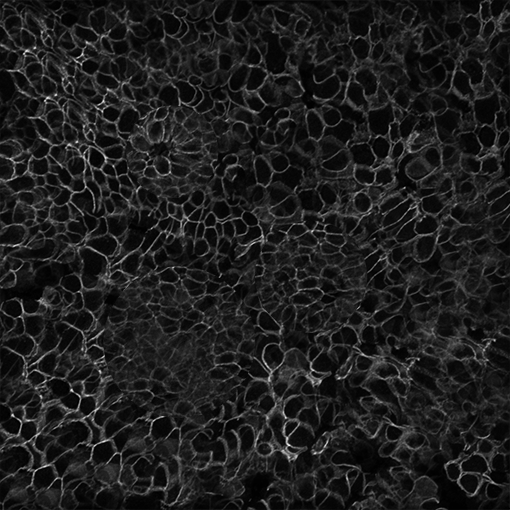
\includegraphics[width=75px, frame]{figures/accuracy_maps/if_fill/adh_dcis_01_dcis_bg.png}
			&
			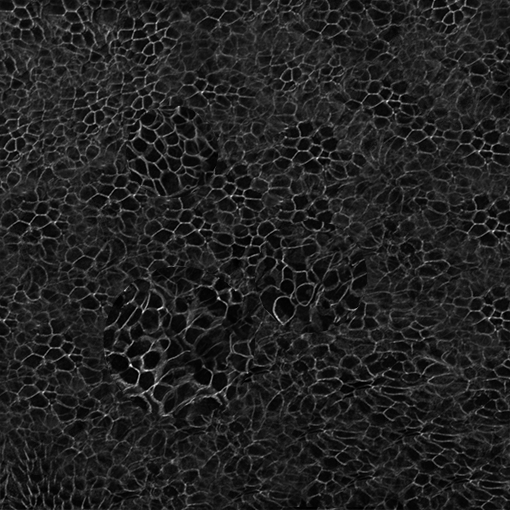
\includegraphics[width=75px, frame]{figures/accuracy_maps/if_fill/adh_dcis_02_adh_bg.png}
			& 
			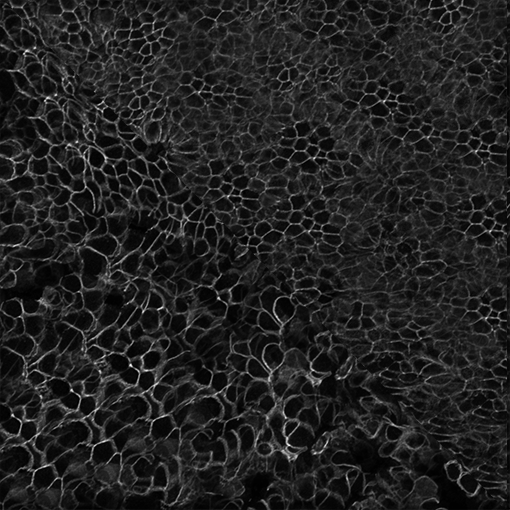
\includegraphics[width=75px, frame]{figures/accuracy_maps/if_fill/adh_dcis_02_adh_top_right.png}
			\\ 
			\hline
			(b)
			&
			Ground Truth
			&
			
\includegraphics[width=75px, frame]{figures/accuracy_maps/ground_truth_brick_gravel_01.png}
			&
			
\includegraphics[width=75px, frame]{figures/accuracy_maps/ground_truth_brick_gravel_02.png}
			& 
			
\includegraphics[width=75px, frame]{figures/accuracy_maps/if_fill/adh_dcis_510.png}
			\\
			\hline
			(c)
			&
			Classified Image
			&
			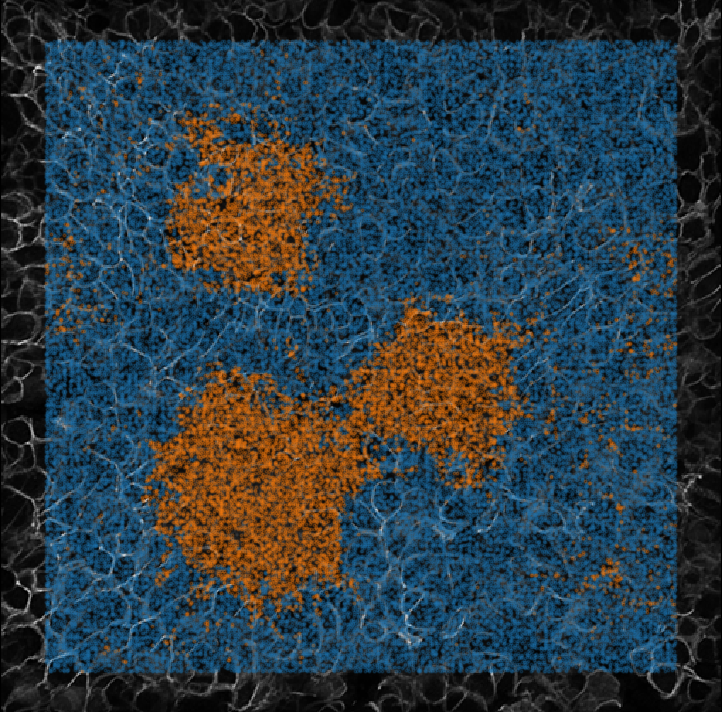
\includegraphics[width=75px, frame]{figures/accuracy_maps/if_fill/adh_dcis_classified_dcis_bg_tight.png}
			&
			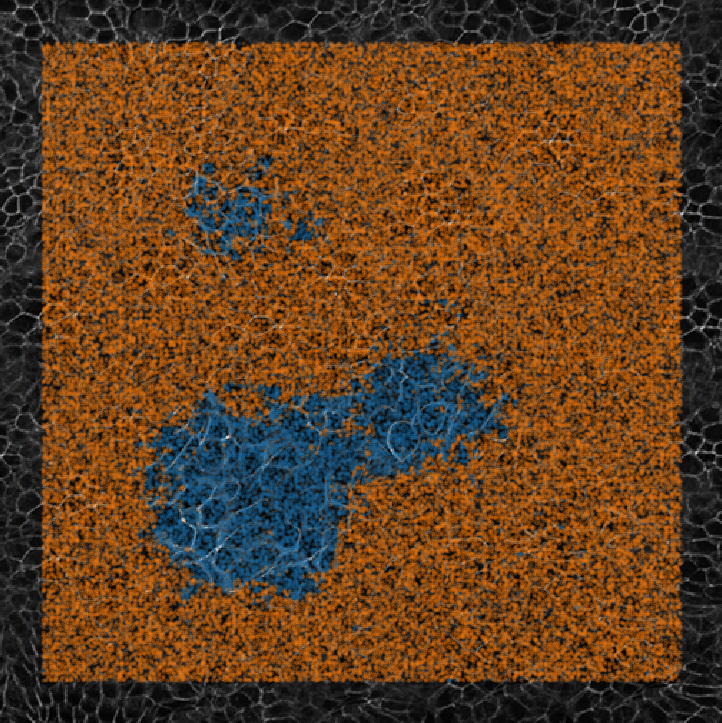
\includegraphics[width=75px, frame]{figures/accuracy_maps/if_fill/adh_dcis_classified_adh_bg_tight.png}
			&
			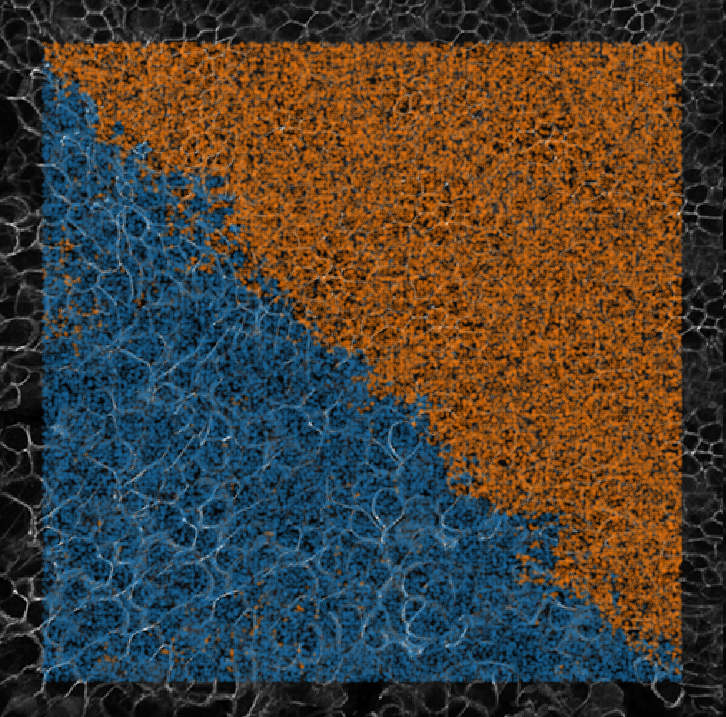
\includegraphics[width=75px, frame]{figures/accuracy_maps/if_fill/adh_dcis_slant_tight.png}
			\\
			\hline
			(d)
			&
			Hyperplasia Accuracy Map
			&
			\includegraphics[width=75px, frame]{figures/accuracy_maps/if_fill/accuracy_dcis_bg__adh_tight-01.pdf}
			&
			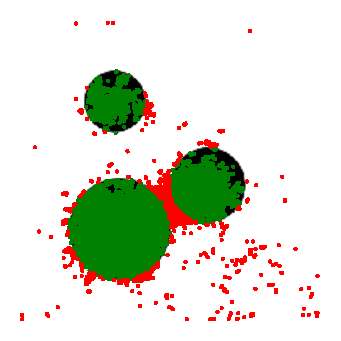
\includegraphics[width=75px, frame]{figures/accuracy_maps/if_fill/accuracy_adh_bg__dcis_tight-01.pdf}
			&
			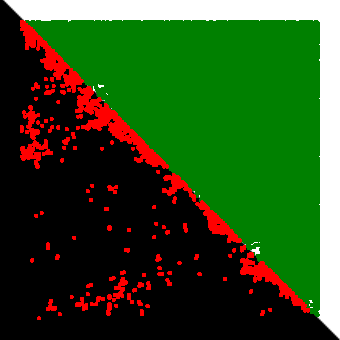
\includegraphics[width=75px, frame]{figures/accuracy_maps/if_fill/accuracy_slant_adh_bg__adh_tight-01.pdf}
			\\
			\hline
			(e)
			&
			Carcinoma Accuracy Map
			&
			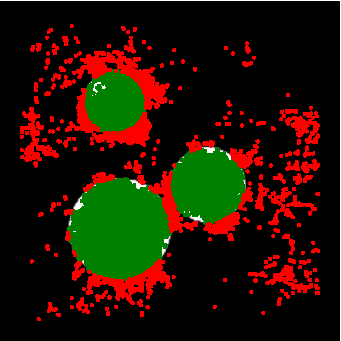
\includegraphics[width=75px, frame]{figures/accuracy_maps/if_fill/accuracy_dcis_bg__dcis_tight-01.pdf}
			&
			\includegraphics[width=75px, frame]{figures/accuracy_maps/if_fill/accuracy_adh_bg__adh_tight-01.pdf}
			&
			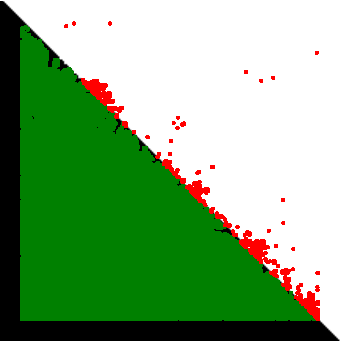
\includegraphics[width=75px, frame]{figures/accuracy_maps/if_fill/accuracy_slant_adh_bg__dcis_tight-01.pdf}
			\\ 
			\hline
			(f)
			&
			Accuracy
			&
			93.17\%
			&
			93.60\%
			&
			96.00\% 
			\\
			\hline
		\end{tabular}\par
	\end{center}
	\bigskip
	\begin{singlespace}
		\textit{Legend} --- \textbf{(a)} Test images comprised of composites of textures derived from \mbox{E-cadherin} staining of human lesions exhibiting characteristic hyperplastic or carcinomic cell patterning. \textbf{(b)} The ideal classification (or ``ground truth'') of the original test image, where black pixels code for the hyperplastic texture and white codes for the carcinomic texture. \textbf{(c)} A random sampling of pixels classified by the PPReCOGG model. Pixels classified as hyperplasia are coded by blue points, and and pixels classified as carcinoma are coded by orange pixels. \textbf{(d)} and \textbf{(e)} Classified pixels are here compared to and overlayed on their ground truth. Pixels which are correctly classified are coded in green, while false-positives are coded in red. \textbf{(f)} Accuracy of the model, as calculated by the quotient of the number of correctly classified pixels and the total number of classified pixels.
	\end{singlespace}
\end{minipage}



\begin{figure}[p]
	\begin{center}
		\caption{Human Lesions as Classified by the PPReCOGG Model \label{fig:pprecogg_human_lesion}}
	\end{center}
	\includegraphics[width=155mm]{figures/human_pprecogg.pdf}
	\begin{singlespace}
		\textit{Legend} --- Sections of human breast biopsies were immunofluorescently stained for E-cadherin and classified using the PPReCOGG model trained on two different early transformed phenotypes, and one background control. \textbf{(a)} Three representative fields of the 512 pixel by 512 pixel images used to train the PPReCOGG model. \textbf{(b)} Fields of breast E-cadherin labelled human breast lesion (left column) were classified by the trained \mbox{PPReCOGG} model (right column). Blue and orange pixels are classified as belonging to a hyperplastic carcinomic regions, respectively. Green pixels are classified as background signal.
	\end{singlespace}
	
\end{figure}
